%%
%% This is file `sample-sigplan.tex',
%% generated with the docstrip utility.
%%
%% The original source files were:
%%
%% samples.dtx  (with options: `sigplan')
%% 
%% Commands for TeXCount
%TC:macro \cite [option:text,text]
%TC:macro \citep [option:text,text]
%TC:macro \citet [option:text,text]
%TC:envir table 0 1
%TC:envir table* 0 1
%TC:envir tabular [ignore] word
%TC:envir displaymath 0 word
%TC:envir math 0 word
%TC:envir comment 0 0

\documentclass[sigplan,screen]{acmart}
%% \documentclass[manuscript,screen,review]{acmart}

%% Rights management information.  
\setcopyright{acmlicensed}
\copyrightyear{2023}
\acmYear{2023}
\acmDOI{XXXXXXX.XXXXXXX}

%% These commands are for a PROCEEDINGS abstract or paper.
\acmConference[Conference acronym 'XX]{Make sure to enter the correct
  conference title from your rights confirmation emai}{June 03--05,
  2018}{Woodstock, NY}
%
%  Uncomment \acmBooktitle if th title of the proceedings is different
%  from ``Proceedings of ...''!
%
%\acmBooktitle{Woodstock '18: ACM Symposium on Neural Gaze Detection,
%  June 03--05, 2018, Woodstock, NY} 
\acmISBN{978-1-4503-XXXX-X/18/06}

\begin{document}

\title{Improvements to the MLCommons Cloudmask Benchmark}


\author{Gregor von Laszewski}
\email{laszewski@gmail.com}
\orcid{0000-0001-9558-179X}
\authornote{MLCommons authorized submitting author}
\affiliation{%
  \institution{University of Virginia}
  \streetaddress{Biocomplexity Institute and Initiative\\
Town Center Four\\
994 Research Park Boulevard}
  \city{Charlottesville}
  \state{VA}
  \postcode{22911}
  \country{USA}
}

\author{Ruchen Gu}
\email{youremail@gmail.com}


%%
%% By default, the full list of authors will be used in the page
%% headers. Often, this list is too long, and will overlap
%% other information printed in the page headers. This command allows
%% the author to define a more concise list
%% of authors' names for this purpose.
\renewcommand{\shortauthors}{von Laszewski, et al.}

%%
%% The abstract is a short summary of the work to be presented in the
%% article.
\begin{abstract}
  A clear and well-documented \LaTeX\ document is presented as an
  article formatted for publication by ACM in a conference proceedings
  or journal publication. Based on the ``acmart'' document class, this
  article presents and explains many of the common variations, as well
  as many of the formatting elements an author may use in the
  preparation of the documentation of their work.
\end{abstract}

%%
%% The code below is generated by the tool at http://dl.acm.org/ccs.cfm.
%% Please copy and paste the code instead of the example below.
%%
\begin{CCSXML}
<ccs2012>
 <concept>
  <concept_id>00000000.0000000.0000000</concept_id>
  <concept_desc>Do Not Use This Code, Generate the Correct Terms for Your Paper</concept_desc>
  <concept_significance>500</concept_significance>
 </concept>
 <concept>
  <concept_id>00000000.00000000.00000000</concept_id>
  <concept_desc>Do Not Use This Code, Generate the Correct Terms for Your Paper</concept_desc>
  <concept_significance>300</concept_significance>
 </concept>
 <concept>
  <concept_id>00000000.00000000.00000000</concept_id>
  <concept_desc>Do Not Use This Code, Generate the Correct Terms for Your Paper</concept_desc>
  <concept_significance>100</concept_significance>
 </concept>
 <concept>
  <concept_id>00000000.00000000.00000000</concept_id>
  <concept_desc>Do Not Use This Code, Generate the Correct Terms for Your Paper</concept_desc>
  <concept_significance>100</concept_significance>
 </concept>
</ccs2012>
\end{CCSXML}

\ccsdesc[500]{Do Not Use This Code~Generate the Correct Terms for Your Paper}
\ccsdesc[300]{Do Not Use This Code~Generate the Correct Terms for Your Paper}
\ccsdesc{Do Not Use This Code~Generate the Correct Terms for Your Paper}
\ccsdesc[100]{Do Not Use This Code~Generate the Correct Terms for Your Paper}

%%
%% Keywords. The author(s) should pick words that accurately describe
%% the work being presented. Separate the keywords with commas.
\keywords{MLCommons, Cloud detection, cloudmesh}

%\received{1 December 2023}
%\received[revised]{12 March 2009}
%\received[accepted]{5 June 2009}

\maketitle

\section{Introduction}

TBD

\cite{cloudmesh-ee}
\cite{cloudmesh-gpu}
\cite{cloudmesh-stopwatch}
\cite{las-2023-escience}
\cite{las-22-arxiv-workflow-cc}
\cite{las-22-mlcommons-science}
\cite{mlperf-training}
\cite{www-mlcommons}
\cite{uva-ondemand}
\cite{www-rivanna}
\cite{www-slurm}




\subsection{Hardware used for this Research}

The benchmarks we present in the next sections have been run on a number of compute resources. This includes not only an HPC at the University of Virginia (UVA) but also a desktop, a laptop, and Google Colab to represent different classes of computing resources that students have access to. We used the following resources:

\begin{itemize}
\item {\bf Rivanna}~\citep{www-rivanna} -- The Rivanna HPC cluster is  a system hosted at the University of Virginia with 15 different  hardware configurations spanning 575 nodes.  There exist 5 different  classes of GPUs on these nodes. The Rivanna HPC follows the  condominium model and continues to receive additions of nodes and  upgrades at various times.
\item {\bf Google Colab}~\cite{google-colab} is a free-to-use interactive computing service offered by Google that provides on-demand access to GPUs and TPUs. Google Colab is designed to be used with machine learning and data analysis \cite{google-colab}. When running with Google Colab, multiple hardware configurations may be provided depending on the instance type. The Pro+ plan allocates an NVIDIA V100 with 53GB of RAM for a GPU configuration. The free  plan only offers 32 GB and a P100 GPU.
\item {\bf Desktop} -- A custom-built desktop with an AMD 5950X processor, 128GB memory, and fast NVMe storage.
\item {\bf Laptop} -- A store-bought laptop with an AMD 5900HX processor, 16GB memory, and NVMe storage.

\end{itemize}


The details of the machines are showcased in Table~\ref{tab:hwoverview}.

\begin{comment}
\begin{table*}[htb]
\begin{verbatim}
17 * servers with 8 a100 80G, 128 AMD EPYC 7742 CPU, 2T Memory, 100Gb Infiniband
 2 * servers with 8 a100 40G, 128 AMD EPYC 7742 CPU, 1T Memory, 100Gb Infiniband
15 * servers with 8 a6000, 48 AMD EPYC 7352 CPU, 250G Memory, 100Gb Infiniband
 2 * servers with 10 rtx2080, 40 Intel(R) Xeon(R) Gold 6148 CPU @ 2.40GHz, 376G Memory, 100Gb Infiniband
 5 * servers with 4 rtx3090, 32 AMD EPYC 7302 CPU 125G Memory, 100Gb Infiniband
12 * servers with 4 v100, 40 Intel(R) Xeon(R) Gold 6148 CPU @ 2.40GHz, 376G Memory, 100Gb Infiniband
 3 * servers with 4 v100, 36 Intel(R) Xeon(R) Gold 6240 CPU @ 2.60GHz, 376G Memory, 100Gb Infiniband
 1 * servers with 4 v100, 28 Intel(R) Xeon(R) Gold 6132 CPU @ 2.60GHz, 187G Memory, 100Gb Infiniband
\end{verbatim}
\end{table*}
\end{comment}


\begin{table*}[htb]
    \caption{Overview of the computing resources.}
    \label{tab:hwoverview}
    \begin{center}
    {\footnotesize
    \begin{tabular}{|l|r|r|r|r|r|r|r|r|}
        \hline
            {\bf Machine}  & {\bf Cores} & {\bf Memory} & {\bf GPU} & {\bf GPU}   &   {\bf Memory} & {\bf \# GPUs} & {\bf \# Nodes}  & {\bf Commissioned} \\ 
                     &  {\bf / Node} & {\bf / Node}  &  & {\bf Total} & {\bf / GPU} & {\bf / Node}     &   {\bf / Node}        &  \\
        \hline
        \hline
        Rivanna (UVA)    & 128 & 2000GB   & 136 & A100 & 80GB &  8  & 17 & Feb 2022 \\
                        & 128 & 1000GB   & 16 & A100 & 40GB &  8  &  2 & Jun 2022  \\  & 48 & 250GB   & 120 & A6000 & 48GB &  8  &  15 & Jun 2022  \\   
                        & 28  & 255GB    & 64 & K80  & 11GB &  8  &  8 & Jun 2018         \\
                        & 28  & 255GB    & 16 & P100 & 12GB &  4  &  4 & Jan 2018         \\
                        & 28  & 188GB    & 4 & V100 & 16GB &  4  &  1 & Feb 2019          \\
                        & 40  & 384GB    & 48 & V100 & 32GB &  4  & 12 & Feb 2021          \\
                        & 36  & 384GB    & 12 & V100 & 32GB &  4  &  3 & Apr 2022          \\
                        &  64 & 128     & 20 & RTX3090   & 24GB    & 4   &  5 & Feb 2023         \\
                        & 40  & 384GB    & 20 & RTX2080TI & 11GB & 10  &  2 & May 2021 \\                        
         \hline
         Google Colab      & -   & 32GB      & & P100      & 16GB    & 1 & - & March 2022 \\
         Google Colab Pro+ & -   & 53GB      & & V100      & 32GB    & 1 & - & March 2022 \\
         \hline
         Desktop 5950X     &  32 & 128GB     & 1& RTX3090   & 24GB    & 1 & 1 & Feb 2022   \\
         \hline
    \end{tabular}
    }
    \end{center}
\end{table*}

\begin{figure}[h]
  \centering
  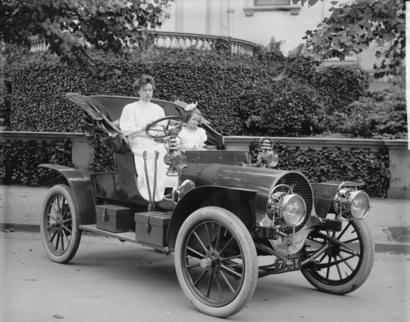
\includegraphics[width=\linewidth]{sample-franklin}
  \caption{1907 Franklin Model D roadster. Photograph by Harris \&
    Ewing, Inc. [Public domain], via Wikimedia
    Commons. (\url{https://goo.gl/VLCRBB}).}
  \Description{A woman and a girl in white dresses sit in an open car.}
\end{figure}

  \cite{Harel79}, a divisible-book such as an anthology or compilation

\section{Acknowledgments}

TBD

\bibliographystyle{ACM-Reference-Format}
\bibliography{sample-base}

%%
%% If your work has an appendix, this is the place to put it.
\appendix


\onecolumn

\section{Naming Convention}

\url{https://sentinels.copernicus.eu/web/sentinel/user-guides/sentinel-3-slstr/naming-convention}

The file naming convention of SLSTR products
(\href{https://earth.esa.int/documents/247904/1964331/Sentinel-3_PDGS_File_Naming_Convention}{see
Sentinel-3 PDGS File Naming Convention for more details}) is identified
by the sequence of fields described below:

\emph{\textbf{MMM\_SL\_L\_TTTTTT\_yyyymmddThhmmss\_YYYYMMDDTHHMMSS\_YYYYMMDDTHHMMSS\_{[}instance
ID{]}\_GGG\_{[}class ID{]}.SEN3}}

where:

\begin{itemize}
\item
  \textbf{MMM}~is the mission ID:

  \begin{itemize}
  \item
    S3A = SENTINEL-3A
  \item
    S3B = SENTINEL-3B
  \item
    S3\_ = for both SENTINEL-3A and 3B
  \end{itemize}
\item
  \textbf{SL}~is the data source/consumer (SL = SLSTR)
\item
  \textbf{L}~is the processing level
(
  \begin{itemize}
  \item
    "0" for Level-0
  \item
    "1" for Level-1
  \item
    "2" for Level-2
  \item
    underscore "\_" if processing level is not applicable
  \end{itemize}
\item
  \textbf{TTTTTT}~is the data Type ID

  \begin{itemize}
  \item
    Level 0 SLSTR data:

    \begin{itemize}
    \item
      "SLT\_\_\_" = ISPs.
    \end{itemize}
  \item
    Level-1 SLSTR data:

    \begin{itemize}
    \item
      "RBT\_\_\_" = TOA Radiances and Brightness Temperature
    \item
      "RBT\_BW" = browse product derived from "RBT\_\_\_".
    \end{itemize}
  \item
    Level-2 SLSTR data:

    \begin{itemize}
    \item
      "WCT\_\_\_" = 2 and 3 channels SST for nadir and along track view
    \item
      "WST\_\_\_" = L2P sea surface temperature
    \item
      "LST\_\_\_" = land surface temp
    \item
      "FRP\_\_\_" = Fire Radiative Power
    \item
      "WST\_BW" = browse product derived from "WST\_\_\_"
    \item
      "LST\_BW" = browse product derived from "LST\_\_\_".
    \end{itemize}
  \end{itemize}
\item
  \textbf{yyyymmddThhmmss}~is the sensing start time
\item
  \textbf{YYYYMMDDTHHMMSS}~is the sensing stop time
\item
  \textbf{YYYYMMDDTHHMMSS}~is the product creation date
\item
  \textbf{{[}instance ID{]}~}consists of 17 characters, either uppercase
  letters or digits or underscores "\_".
\end{itemize}

\begin{quote}
The instance id fields include the following cases, applicable as
indicated:

\begin{enumerate}
\item Instance ID for the instrument data products disseminated in
"stripes":

Duration,"\_", cycle number, "\_", relative orbit number,"\_", 4
underscores "\_", i.e.\\
DDDD\_CCC\_LLL\_\_\_\_\_\\
\item Instance ID for the instrument data products ~\\
disseminated in "frames":\\
Duration, "\_", cycle number, "\_", relative orbit number, "\_", frame
along track coordinate, i.e.\\
DDDD\_CCC\_LLL\_FFFF\\
\item Instance ID for the instrument data products disseminated in
"tiles".\\
Two sub-cases are applicable:

a) tile covering the whole globe:\\
\hspace*{0.333em}\hspace*{0.333em}\hspace*{0.333em}\hspace*{0.333em}\hspace*{0.333em}
"GLOBAL\_\_\_\_\_\_\_\_\_\_\_"\\

b) tile cut according to specific\\
geographical criteria:\\
Tile Identifier\\
ttttttttttttttttt\\
\item Instance ID for auxiliary data:\\
17 underscores "\_"

\end{enumerate}
\end{quote}

\begin{itemize}
\item
  \textbf{GGG}~identifies the centre which generated the file
\item
  \textbf{{[}class ID{]}}~identifies the class ID for instrument data
  products with conventional sequence~\textbf{P\_XX\_NNN}~where:

  \begin{itemize}
  \item
    P indicates the platform (O for operational, F for reference, D for
    development, R for reprocessing)
  \item
    XX indicates the timeliness of the processing workflow (NR for NRT,
    ST for STC, NT for NTC)
  \item
    NNN indicates the baseline collection or data usage.
  \end{itemize}
\item
  \textbf{.SEN3}~is the filename extension
\end{itemize}

Example of filename:


\verb|S3A_SL_2_LST____20151229T095534_20151229T114422_20160102T150019_6528_064_365______LN2_D_NT_001.SEN3|

\section{Inference Files}

\begin{verbatim}
S3A_SL_1_RBT____20191001T113221_20191001T113521_20191002T153211_0179_050_023_1980_LN2_O_NT_003.hdf
S3A_SL_1_RBT____20191002T124409_20191002T124709_20191003T180638_0180_050_038_1800_LN2_O_NT_003.hdf
S3A_SL_1_RBT____20191002T124709_20191002T125009_20191003T180806_0179_050_038_1980_LN2_O_NT_003.hdf
S3A_SL_1_RBT____20191002T125609_20191002T125909_20191003T181226_0179_050_038_2520_LN2_O_NT_003.hdf
S3A_SL_1_RBT____20191003T122059_20191003T122359_20191004T173532_0179_050_052_1980_LN2_O_NT_003.hdf
S3A_SL_1_RBT____20191003T122659_20191003T122959_20191004T173822_0179_050_052_2340_LN2_O_NT_003.hdf
S3A_SL_1_RBT____20191004T114848_20191004T115148_20191005T172918_0179_050_066_1620_LN2_O_NT_003.hdf
S3A_SL_1_RBT____20191004T115148_20191004T115448_20191005T173023_0179_050_066_1800_LN2_O_NT_003.hdf
S3A_SL_1_RBT____20191004T115448_20191004T115748_20191005T173129_0180_050_066_1980_LN2_O_NT_003.hdf
S3A_SL_1_RBT____20191004T120048_20191004T120348_20191005T173344_0179_050_066_2340_LN2_O_NT_003.hdf
S3A_SL_1_RBT____20191005T112237_20191005T112537_20191006T161503_0179_050_080_1620_LN2_O_NT_003.hdf
S3A_SL_1_RBT____20191005T112537_20191005T112837_20191006T161611_0179_050_080_1800_LN2_O_NT_003.hdf
S3A_SL_1_RBT____20191005T112837_20191005T113137_20191006T161718_0179_050_080_1980_LN2_O_NT_003.hdf
S3A_SL_1_RBT____20191006T105626_20191006T105926_20191007T153322_0179_050_094_1620_LN2_O_NT_003.hdf
S3A_SL_1_RBT____20191006T124025_20191006T124325_20191007T170714_0179_050_095_1800_LN2_O_NT_003.hdf
S3A_SL_1_RBT____20191006T125225_20191006T125525_20191007T171148_0179_050_095_2520_LN2_O_NT_003.hdf
S3A_SL_1_RBT____20191007T121414_20191007T121714_20191009T123433_0179_050_109_1800_LN2_O_NT_003.hdf
S3A_SL_1_RBT____20191007T121714_20191007T122014_20191009T123540_0179_050_109_1980_LN2_O_NT_003.hdf
S3A_SL_1_RBT____20191007T122614_20191007T122914_20191009T123903_0179_050_109_2520_LN2_O_NT_003.hdf
S3A_SL_1_RBT____20191008T114803_20191008T115103_20191009T162306_0179_050_123_1800_LN2_O_NT_003.hdf
S3A_SL_1_RBT____20191008T115103_20191008T115403_20191009T162431_0179_050_123_1980_LN2_O_NT_003.hdf
S3A_SL_1_RBT____20191008T115703_20191008T120003_20191009T162735_0179_050_123_2340_LN2_O_NT_003.hdf
S3A_SL_1_RBT____20191009T112453_20191009T112753_20191010T171844_0180_050_137_1980_LN2_O_NT_003.hdf
S3A_SL_1_RBT____20191009T195549_20191009T195849_20191011T011836_0179_050_142_2340_LN2_O_NT_003.hdf
S3A_SL_1_RBT____20191012T114719_20191012T115019_20191013T162441_0179_050_180_1980_LN2_O_NT_003.hdf
S3A_SL_1_RBT____20191014T123257_20191014T123557_20191015T172725_0179_050_209_1800_LN2_O_NT_003.hdf
S3A_SL_1_RBT____20191014T123557_20191014T123857_20191015T172851_0179_050_209_1980_LN2_O_NT_003.hdf
S3A_SL_1_RBT____20191014T124457_20191014T124757_20191015T173252_0179_050_209_2520_LN2_O_NT_003.hdf
S3A_SL_1_RBT____20191015T120646_20191015T120946_20191016T160534_0179_050_223_1800_LN2_O_NT_003.hdf
S3A_SL_1_RBT____20191015T120946_20191015T121246_20191016T160700_0179_050_223_1980_LN2_O_NT_003.hdf
S3A_SL_1_RBT____20191015T121546_20191015T121846_20191016T160934_0179_050_223_2340_LN2_O_NT_003.hdf
S3A_SL_1_RBT____20191017T130723_20191017T131023_20191018T181427_0179_050_252_2520_LN2_O_NT_003.hdf
S3A_SL_1_RBT____20191017T194820_20191017T195120_20191019T014123_0180_050_256_2340_LN2_O_NT_003.hdf
S3A_SL_1_RBT____20191018T122912_20191018T123212_20191019T172627_0180_050_266_1800_LN2_O_NT_003.hdf
S3A_SL_1_RBT____20191019T120301_20191019T120601_20191020T172539_0179_050_280_1800_LN2_O_NT_003.hdf
S3A_SL_1_RBT____20191019T120601_20191019T120901_20191020T172659_0179_050_280_1980_LN2_O_NT_003.hdf
S3A_SL_1_RBT____20191019T121201_20191019T121501_20191020T172947_0179_050_280_2340_LN2_O_NT_003.hdf
S3A_SL_1_RBT____20191020T113650_20191020T113950_20191021T155904_0179_050_294_1800_LN2_O_NT_003.hdf
S3A_SL_1_RBT____20191020T113950_20191020T114250_20191021T160028_0179_050_294_1980_LN2_O_NT_003.hdf
S3A_SL_1_RBT____20191022T122528_20191022T122828_20191023T162316_0179_050_323_1800_LN2_O_NT_003.hdf
S3A_SL_1_RBT____20191022T122828_20191022T123128_20191023T162424_0179_050_323_1980_LN2_O_NT_003.hdf
S3A_SL_1_RBT____20191023T115917_20191023T120217_20191024T181537_0179_050_337_1800_LN2_O_NT_003.hdf
S3A_SL_1_RBT____20191023T120217_20191023T120517_20191024T181700_0179_050_337_1980_LN2_O_NT_003.hdf
S3A_SL_1_RBT____20191023T120817_20191023T121117_20191024T181932_0179_050_337_2340_LN2_O_NT_003.hdf
S3A_SL_1_RBT____20191024T113606_20191024T113906_20191025T164619_0180_050_351_1980_LN2_O_NT_003.hdf
S3A_SL_1_RBT____20191024T114206_20191024T114506_20191025T164855_0179_050_351_2340_LN2_O_NT_003.hdf
S3A_SL_1_RBT____20191026T122143_20191026T122443_20191027T165912_0179_050_380_1800_LN2_O_NT_003.hdf
S3A_SL_1_RBT____20191026T122443_20191026T122743_20191027T170026_0179_050_380_1980_LN2_O_NT_003.hdf
S3A_SL_1_RBT____20191026T123343_20191026T123643_20191027T170426_0180_050_380_2520_LN2_O_NT_003.hdf
S3A_SL_1_RBT____20191027T115532_20191027T115832_20191028T171044_0179_051_009_1800_LN2_O_NT_003.hdf
S3A_SL_1_RBT____20191027T115832_20191027T120132_20191028T171322_0179_051_009_1980_LN2_O_NT_003.hdf
S3A_SL_1_RBT____20191027T120432_20191027T120732_20191028T171546_0179_051_009_2340_LN2_O_NT_003.hdf
S3A_SL_1_RBT____20191028T131020_20191028T131320_20191029T181138_0179_051_024_1800_LN2_O_NT_003.hdf
S3A_SL_1_RBT____20191029T124409_20191029T124709_20191030T172048_0179_051_038_1800_LN2_O_NT_003.hdf
S3A_SL_1_RBT____20191029T125609_20191029T125909_20191030T172609_0179_051_038_2520_LN2_O_NT_003.hdf
S3A_SL_1_RBT____20191001T230116_20191001T230416_20191003T022222_0179_050_030_0900_LN2_O_NT_003.hdf
S3A_SL_1_RBT____20191002T223505_20191002T223805_20191004T031930_0179_050_044_0900_LN2_O_NT_003.hdf
S3A_SL_1_RBT____20191003T220854_20191003T221154_20191005T030445_0179_050_058_0900_LN2_O_NT_003.hdf
S3A_SL_1_RBT____20191003T234353_20191003T234653_20191005T041723_0179_050_059_0540_LN2_O_NT_003.hdf
S3A_SL_1_RBT____20191004T231742_20191004T232042_20191006T041726_0179_050_073_0540_LN2_O_NT_003.hdf
S3A_SL_1_RBT____20191005T225731_20191005T230031_20191007T024922_0179_050_087_0900_LN2_O_NT_003.hdf
S3A_SL_1_RBT____20191006T223121_20191006T223421_20191008T021301_0179_050_101_0900_LN2_O_NT_003.hdf
S3A_SL_1_RBT____20191007T014419_20191007T014719_20191008T061144_0179_050_103_0360_LN2_O_NT_003.hdf
S3A_SL_1_RBT____20191007T202711_20191007T203011_20191009T155246_0179_050_114_1080_LN2_O_NT_003.hdf
S3A_SL_1_RBT____20191007T220510_20191007T220810_20191010T073003_0179_050_115_0900_LN2_O_NT_003.hdf
S3A_SL_1_RBT____20191008T114503_20191008T114803_20191009T162144_0179_050_123_1620_LN2_O_NT_003.hdf
S3A_SL_1_RBT____20191009T093753_20191009T094053_20191010T151007_0179_050_136_1620_LN2_O_NT_003.hdf
S3A_SL_1_RBT____20191009T111853_20191009T112153_20191010T171717_0179_050_137_1620_LN2_O_NT_003.hdf
S3A_SL_1_RBT____20191010T071243_20191010T071543_20191011T114643_0179_050_149_0540_LN2_O_NT_003.hdf
S3A_SL_1_RBT____20191010T105242_20191010T105542_20191011T160548_0179_050_151_1620_LN2_O_NT_003.hdf
S3A_SL_1_RBT____20191011T014035_20191011T014335_20191012T060733_0179_050_160_0360_LN2_O_NT_003.hdf
S3A_SL_1_RBT____20191011T102631_20191011T102931_20191012T152504_0180_050_165_1620_LN2_O_NT_003.hdf
S3A_SL_1_RBT____20191011T184527_20191011T184827_20191013T002531_0179_050_170_1260_LN2_O_NT_003.hdf
S3A_SL_1_RBT____20191012T181916_20191012T182216_20191013T230919_0179_050_184_1260_LN2_O_NT_003.hdf
S3A_SL_1_RBT____20191013T172106_20191013T172406_20191014T215723_0179_050_197_5400_LN2_O_NT_003.hdf
S3A_SL_1_RBT____20191013T175305_20191013T175605_20191014T222812_0180_050_198_1260_LN2_O_NT_003.hdf
S3A_SL_1_RBT____20191013T225003_20191013T225303_20191015T030239_0179_050_201_0900_LN2_O_NT_003.hdf
S3A_SL_1_RBT____20191014T222352_20191014T222652_20191016T015710_0179_050_215_0900_LN2_O_NT_003.hdf
S3A_SL_1_RBT____20191015T102247_20191015T102547_20191016T142544_0179_050_222_1620_LN2_O_NT_003.hdf
S3A_SL_1_RBT____20191015T120346_20191015T120646_20191016T160531_0179_050_223_1620_LN2_O_NT_003.hdf
S3A_SL_1_RBT____20191015T215741_20191015T220041_20191017T010323_0179_050_229_0900_LN2_O_NT_003.hdf
S3A_SL_1_RBT____20191016T075436_20191016T075736_20191017T123959_0179_050_235_0360_LN2_O_NT_003.hdf
S3A_SL_1_RBT____20191016T095636_20191016T095936_20191017T152606_0179_050_236_1620_LN2_O_NT_003.hdf
S3A_SL_1_RBT____20191016T195331_20191016T195631_20191018T012929_0179_050_242_1080_LN2_O_NT_003.hdf
S3A_SL_1_RBT____20191017T004429_20191017T004729_20191018T060449_0179_050_245_0360_LN2_O_NT_003.hdf
S3A_SL_1_RBT____20191018T222008_20191018T222308_20191020T032233_0179_050_272_0900_LN2_O_NT_003.hdf
S3A_SL_1_RBT____20191019T120001_20191019T120301_20191020T172512_0179_050_280_1620_LN2_O_NT_003.hdf
S3A_SL_1_RBT____20191019T215357_20191019T215657_20191021T014757_0179_050_286_0900_LN2_O_NT_003.hdf
S3A_SL_1_RBT____20191020T194947_20191020T195247_20191022T003158_0179_050_299_1080_LN2_O_NT_003.hdf
S3A_SL_1_RBT____20191021T004044_20191021T004344_20191022T051308_0180_050_302_0360_LN2_O_NT_003.hdf
S3A_SL_1_RBT____20191023T115617_20191023T115917_20191024T181537_0180_050_337_1620_LN2_O_NT_003.hdf
S3A_SL_1_RBT____20191023T201213_20191023T201513_20191025T014837_0179_050_342_1080_LN2_O_NT_003.hdf
S3A_SL_1_RBT____20191023T215012_20191023T215312_20191025T023107_0179_050_343_0900_LN2_O_NT_003.hdf
S3A_SL_1_RBT____20191025T003700_20191025T004000_20191026T054924_0180_050_359_0360_LN2_O_NT_003.hdf
S3A_SL_1_RBT____20191027T101133_20191027T101433_20191028T144445_0179_051_008_1620_LN2_O_NT_003.hdf
S3A_SL_1_RBT____20191027T214628_20191027T214928_20191029T013217_0179_051_015_0900_LN2_O_NT_003.hdf
S3A_SL_1_RBT____20191029T003315_20191029T003615_20191030T050058_0179_051_031_0360_LN2_O_NT_003.hdf
S3A_SL_1_RBT____20191029T223505_20191029T223805_20191031T015742_0179_051_044_0900_LN2_O_NT_003.hdf
S3A_SL_1_RBT____20191030T220854_20191030T221154_20191101T025713_0179_051_058_0900_LN2_O_NT_003.hdf
S3A_SL_1_RBT____20191031T231742_20191031T232042_20191102T034613_0179_051_073_0540_LN2_O_NT_003.hdf
\end{verbatim}
\end{document}
\endinput
